\chapter{Eigen Onderzoek}
\label{ch:research}

Alvorens cryptocurrencies aan te kopen, is het van vitaal belang om te weten wat je koopt. Het is aan te raden om te beginnen met het verhaal van Bitcoin en de geschiedenis van de blockchain technologie, want beide hebben een grote impact op de toekomst van de financi{\"e}le sector en de samenleving in haar geheel. Het eigen proces van informatie verzamelen is essentieel om te begrijpen waaraan je deelneemt en waarom je er {\"u}berhaupt aan zou (moeten) willen deelnemen. 

Hierbij is het belangrijk om vooral rustig en kritisch te blijven nadenken, het overzicht te behouden, en bewust te zijn van de emoties die die spelen.

\section{Plan van aanpak}
Starters adviseren wij een holistische aanpak bij het leren over cryptocurrencies en blockchain technologie. 

Bitcoin en blockchain vormen het begin van een (r)evolutie. Een revolutie op het gebied van waarde-transacties. Het is dan ook cruciaal dat je de algemene principes achter Bitcoin en blockchain begrijpt alvorens je je inlaat met specifieke cryptocurrency-projecten. Een logische volgende stap kan zijn de verkenning van een aantal van de alternatieve cryptocurrencies (altcoins). Hieronder volgen aanwijzingen om zelf op onderzoek uit te gaan.\medskip

    \begin{tipbox}{Tip}
        In \cref{app:A} vind je een breed scala aan bronnen (\cref{tab:research_data,tab:social_infrastructure,tab:marketinsight_analyses,tab:learning_tools_general,tab:security_tools}), die wij in de loop der tijd hebben gebruikt om te leren over Bitcoin, blockchain, cryptocurrency, geld en economie.
    \end{tipbox}\medskip

Verdere informatie kan worden opgevraagd bij de talloze andere mensen in de community, men kan op social media en andere kanalen zoeken, video's bekijken, onderzoeksrapporten lezen en nog veel meer. De Cryptomanual en de   \href{https://cryptomanuals.com/5-videos-to-start-with-bitcoin}{website} zijn daar het perfecte startpunt voor. 
\medskip
   
\section{Fundamentele Analyses}
\label{sec:fundamentalanalysis}

Bij beleggingen in bijvoorbeeld bedrijfs-aandelen is een fundamentele analyse van essentieel belang. De financi{\"e}le jaarverslagen, bijbehorende prestaties en cijfers van de voorgaande jaren zijn essentieel om met vertrouwen over te gaan tot investeren. Middels een gedegen analyse krijgt men zicht op de kwaliteit en soliditeit van een investering en beperkt men de risico's. De investeerder bouwt zodoende meer kennis en zelfvertrouwen op m.b.t. beleggingen en daarbij relevante beslissingen. 

Zo leert men meer over de kwaliteit en soliditeit van een investering en worden de risico's beperkt. Tegelijkertijd wordt er gebouwd aan meer kennis en zelfvertrouwen bij de investeerders met betrekking tot het beleggen en de beslissingen die daar allemaal bij komen kijken.\medskip

Financi{\"e}le rapporten en 'track-records' (geschiedenis wat betreft resultaten) zijn er nog nauwelijks betreffende beleggingen in cryptocurrency- en open blockchain-projecten. Wel kun je veel on-chain data vinden van open blockchain-projecten, maar deze gegevens goed opvatten is niet voor iedereen weggelegd. Veel mensen baseren om deze redenen hun beslissingen op beloftes, speculatie of hype. In deze sector wordt men heel gemakkelijk enthousiast over een bepaald project, wat vaak tot gevolg heeft dat objectief onderzoek achterwege wordt gelaten. Onderwerp daarom de volgende aspecten aan een onderzoek alvorens te investeren in een crypto-project.

\begin{enumerate}

    \item \textbf{Technologische Grondslag}
    \begin{itemize}
        \item Hoe sterk of innovatief is de technologie?
        \item Zijn er bekende bugs, netwerkproblemen of andere kwetsbaarheden?
        \item Hoe goed is de code-base? Kijk eventueel op GitHub.
        \item Is het project op Ethereum of een ander platform gebouwd?
        \item Wat is de afweging tussen snelheid, schaalbaarheid en veiligheid?
    \end{itemize}
    \item \textbf{Relevantie}
    \begin{itemize}
        \item Wat is de bruikbaarheid op korte termijn en het nut op lange termijn?
        \item Lost dit project en de bijbehorende cryptocurrency een probleem op? 
        \item Is hier wel een cryptocurrency voor nodig?
        \item Is de voorgestelde oplossing beter dan de huidige oplossingen? Waarom (niet)?
        \item Zal er vraag zijn naar naar de uitgegeven cryptocurrency of token? 
    \end{itemize}
    \item \textbf{Development Team}
    \begin{itemize}
        \item Heeft dit project een toegewijd ontwikkelingsteam?
        \item Hoe sterk zijn de referenties van dit team? 
        \item Wat is de ervaring van het core-team?  
        \item Wordt er actief een bijdrage geleverd vanuit de community? Controleer eventueel de project-geschiedenis op GitHub.
        \item Hoe wordt het project gefinancierd?
      
    \end{itemize}
    \item \textbf{Community}
    \begin{itemize}
        \item Gaat er een proactieve en sympathieke community schuil achter dit project?
     
    \end{itemize}
    \item \textbf{Bestuur}
    \begin{itemize}
        \item Lopen de lijnen binnen het project gecentraliseerd of gedecentraliseerd? Met andere woorden, wie bepaald het beleid en de doelen? Heeft de community hier invloed op?
         \item Hoeveel van de coins hebben de oprichters zelf in bezit?
        \item Is het project of de code hiervan open-source en inzichtelijk?
        \item Hoe is de financiering opgezet?
          \item Is er een marketing strategie?
        \end{itemize}
\end{enumerate}

    \medskip
    \begin{tipbox}{\textbf{Tip}}
    Nadat je account is aangemaakt bij \href{https://www.coinbase.com/join/51954a2b26a1bcc484000015}{Coinbase} kun je direct je eerste gratis cryptocurrencies verdienen terwijl je er meer over leert in een paar video's.
    \tcblower 
 Gelijk aan de slag met \href{https://www.coinbase.com/earn}{Coinbase Earn}
    \end{tipbox}
    \medskip

Hoe kom je aan deze informatie en welke bronnen boor je daarvoor aan? \href{https://www.coinmarketcap.com/}{CoinMarketCap} of \href{https://www.coingecko.com}{CoinGecko} geven een goed totaaloverzicht van de cryptocurrencymarkt. Naast informatie over de totale marktkapitalisatie, bieden ze inzicht in tal van andere indicatoren - van zowel cryptocurrency projecten als de markt als geheel.
Daarnaast bieden ze ook links naar de projectwebsite, social feeds, chats en de broncode. Voor de fundamentele analyse is de primaire bron van informatie voor startende projecten vaak het ontwikkelingsrapport of de whitepaper van het project die door het ontwikkelingsteam is gepubliceerd. Je vindt de whitepapers op de respectievelijke websites. De whitepapers schetsen de visie, missie, probleemstelling, voorgestelde oplossing en technische eigenschappen van het project en de token. In aanvulling op een whitepaper kun je informatie zoeken over activiteiten van ontwikkelaars en gemeenschap. Een goed startpunt vormen de offici{\"e}le website, sociale media en andere communicatiekanalen die het project heeft opgezet.\medskip

\medskip

\begin{cryptobox}{STATE OF THE DAPPS}

    State of the DAPPs is een non-profit website van alle gedecentraliseerde applicaties (ook wel 'DApps' genoemd) die op verschillende blockchains draaien. State of the DApps werd oorspronkelijk ontworpen om op Ethereum ontwikkelde projecten te categoriseren en te tonen, maar tegenwoordig wordt ook ondersteuning voor EOS, POA en Steem geboden. De inspiratie voor State of the DApps kwam van FreshMeat, nu bekend als FreeCode. 
    
    Specifiek aan Linux-gebruikers biedt FreeCode een optimale referentie en inventarisatie van alle open-source applicaties, spellen en bronnen voor Linux. State of the DApps geeft projecten weer op het gebied van gezondheid, games, virtual reality, kunstmatige intelligentie, onderwijs, gegevensopslag, arbeidsmarkt et cetera. 
    
    \tcblower
    Leer meer over DAPPs op; \href{https://www.stateofthedapps.com}{State of the DAPPS}.

\end{cryptobox}

\medskip

\subsection*{Project voortgang en ontwikkeling}
Het is belangrijk om de vooruitgang van projecten te volgen om te beoordelen of de gestelde doelen, tijdschema's en deadlines serieus genomen worden en of de communicatie transparant is. Andere informatiebronnen zijn Reddit, Bitcointalk en video- en blogsites. Meerdere bronnen raadplegen is een betrouwbare manier om informatie en feedback vanuit de community te verzamelen. Dergelijk onderzoek zorgt voor een beter begrip van wat er speelt binnen een community, met welke vragen mensen zitten en hoeveel draagkracht er is. Lees vooral veel artikelen en bekijk de nodige videos's, want daarmee ontwikkel je persoonlijke inzichten en vaardigheden. Dit alles vormt uiteindelijk de basiskennis waarop jij je besluit baseert om al dan niet te investeren.

    \bigskip
    \begin{tipbox}{\textbf{Tip}}
        De cryptocurrency wereld leeft op Twitter! Er zijn tal van alternatieven waaraan op dit moment gewerkt wordt, maar momenteel is Twitter 'the place to be'. Wil je op de hoogte blijven van de nieuwste ontwikkelingen binnen de cryptocurrency en de economische wereld? Kijk dan eens naar wie en welke projecten wij allemaal volgen.
        \tcblower
        \href{https://twitter.com/cryptomanuals}{Follow the Rabbit} op Twitter.
    \end{tipbox}

 \newpage

\section{Coin metrics}
De term 'coin metrics' verwijst naar meetbare gegevens in relatie tot cryptocurrency projecten. Deze data zijn geaggregeerd op websites zoals CoinMarketCap, CoinGecko, en CoinCheckUp. Het gaat hier om verschillende parameters waarvan het nuttig is om te weten waar ze voor staan en wat ze inhouden.  

\begin{enumerate}
    \item \textbf{Aanbod}
    \begin{itemize}
        \item Hoeveel tokens komen er maximaal in circulatie?  
        \item Wat is het huidige aanbod? Hoeveel daarvan circuleert?
        \item Wat is het totale aanbod?
        \item Hoe zijn de tokens verdeeld over investeerders, eigenaren en community.
    \end{itemize}
    \item \textbf{Algoritme}
    \begin{itemize}
        \item Block- en confirmatietijden.
        \item Wat is het consensus mechanisme? 'Proof of work', 'Proof of Stake' of iets totaal anders?
         \item Wordt er gebruik gemaakt van deflatie, inflatie of een ander mechanisme?
            \end{itemize}
    \item \textbf{Marktkapitalisatie, Handelsvolume en Liquiditeit}
    \begin{itemize}
        \item Raadpleeg 'Coin Metrics' op platformen zoals genoemd in \cref{tab:marketinsight_analyses}.
        \item Raadpleeg de ratio's inzake dagelijks handelsvolume en marktkapitalisatie.
    \end{itemize}
\end{enumerate}

\section{Technische Analyses}
\label{sec:technicalanalysis}

Technische analyse wordt vooral gebruikt door traders om de prijs van beleggingen te beoordelen en investeringskansen te vinden. Bij technische analyse worden statistieken verzameld uit de handelsactiviteiten, zoals koersfluctuatie en verhandeld volume. In tegenstelling tot fundamentele analisten (die de intrinsieke waarde van een effect - in dit geval een cryptocurrency - proberen te evalueren), richten technische analisten zich op grafieken van koersbewegingen; zij gebruiken verschillende analytische instrumenten om de kracht of zwakte van een cryptocurrency te beoordelen. Zij zijn van mening dat koerswijzigingen en handelsactiviteiten in het verleden betere indicatoren dan de intrinsieke waarde van de cryptocurrencies zelf. Technische analisten zijn van mening dat de fundamentele waarde volgens dit principe is inbegrepen in de koerswijzigingen van de betreffende cryptocurrency.\medskip

Ervaren traders zijn handig in het gebruiken van tools bij de analyse van grafieken; deze grondige technische analyse is de basis voor hun aankoop- en verkoop-beslissingen. Als je geen ervaring hebt met technische analyse, kun je de basisaspecten ervan aanleren om het optimale instap- of uitstapmoment in de volatiele markt van de cryptocurrencies beter te kunnen beoordelen. Deze kennis kun je vervolgens weer toepassen op andere  markten.

    \medskip
    \begin{tipbox}{Tip}
    Leer meer over de meest populaire trading-indicatoren zoals de Bollinger Bands (BB), Relative Strength Index (RSI) en Moving Average Convergence Divergence (MACD) in \href{https://medium.com/@harrynicholls/7-popular-technical-indicators-and-how-to-use-them-to-increase-your-trading-profits-7f13ffeb8d05}{dit artikel}.  
    \tcblower
    Ga naar \href{https://www.tradingview.com/}{TradingView} en voeg cryptocurrencies toe aan jouw 'watchlist'.
    \end{tipbox}
    \medskip    

Er zijn verschillende platformen die je kunt gebruiken voor technische analyse. \href{https://www.tradingview.com/}{TradingView} biedt een gratis platform aan om grafieken van verschillende markten te analyseren. Hier vind je een grote community van actieve traders. Ze publiceren er hun ide{\"e}en en inzichten. \href{https://coincheckup.com/}{CoinCheckUp} is een onderzoeksplatform dat verschillende tools aanbiedt voor het samenstellen van je eigen analyse. Zo zijn er nog een aantal bronnen en platformen die je kunt gebruiken, zie \cref{app:A}, \cref{tab:marketinsight_analyses}. 


\medskip

\section{Markt Psychologie \& Markt Sentiment}
Technische analyse stelt je in staat om het spel van vraag en aanbod bij bepaalde prijsniveaus goed te volgen. Maar ook marktpsychologie en marktsentiment spelen een belangrijke rol. Voor elk (digitaal) goed bestaat de markt namelijk uit de vraag en het aanbod van mensen, bedrijven en instellingen van over de hele wereld welke zich zowel rationeel als irrationeel gedragen. Het erkennen van dit feit zal van vitaal belang zijn voor jouw succes.

    \medskip
    \begin{figure}
        \centering
        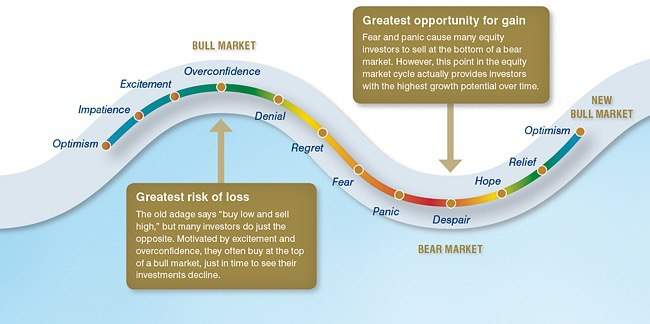
\includegraphics[width=.95\textwidth]{img/ch-investing/bear_bullmarket.jpg}
        \caption[Bear and Bull Markets and Market Psychology]{Marktpsychologie is de drijvende kracht achter de zogenaamde \say{bear} and \say{bull} markten. In elke fase van de cyclus zijn er beslissingen te nemen door investeerders. Achterliggende emoties in de markt spelen hierbij een grote rol.}
        \label{fig:bear_bullmarket}
        \source{Brightscope; \textit{Research and Data.}}
    \end{figure}
    \medskip

\subsection{Bull Markt}
Je spreekt van een 'Bull Market' als er angst bestaat de spreekwoordelijke boot te missen (FOMO ofwel 'Fear of Missing Out'), waarbij grote winsten aan je neus voorbij dreigen te gaan. FOMO kan uiteindelijk leiden tot overgewaardeerde prijzen van cryptocurrencies. De handelsvolumes schieten omhoog en iedereen koopt zich in en doet mee aan de hype. Ook hier spelen marktsentiment en marktpsychologie een grote rol. Het gedrag van onervaren beleggers wordt in dat geval sterk be{\"i}nvloed door een stortvloed aan positief nieuws, waardoor er een feedback-cyclus ontstaat. Aan het eind van een bull markt daalt de prijs van de overgewaardeerde aandelen - de prijzen-bubbel - in snel tempo. Dit brengt extra risico's met zich mee: het kan resulteren in een drastisch verlies in waarde - als je de 'exit points' van je beleggingen niet zorgvuldig hebt getimed.\medskip

\subsection{Bear Markt}
Je spreekt van een 'Bear Market' wanneer angst, onzekerheid en twijfels toeslaan (FUD: Fear, Uncertainty \& Doubt). Bitcoin en cryptocurrencies komen dan vooral negatief in het nieuws, hetgeen een verdere negatieve spiraal kan veroorzaken (massale verkoop van cryptocurrencies). Het negatieve marktsentiment kan zeer lang aanhouden, waardoor mensen zogenaamde 'weak hands' kunnen krijgen. Dit betekent dat (grote) posities crypto's vroegtijdig verkocht worden omdat het vertrouwen in de investering verloren gaat. Bij mensen die hun acties baseren op wat ze zien of horen van anderen, ontbreekt het fundamentele onderzoek dat nu juist aan de basis ligt van zelfvertrouwen in eigen aankopen en eventuele verkopen van de investeringen. 

    \medskip
    \begin{tipbox}{Tip}
    Wanneer het sentiment onder beleggers zich op een dieptepunt bevindt, de prijzen instorten en iedereen aan het verkopen slaat, denk juist dan nog eens goed na. Dit is wellicht net het moment om te kopen. Probeer het laagste punt niet te timen maar spreid de momenten van aankoop en start met lage bedragen. 
    \end{tipbox}\medskip
    \medskip

Een bear market is bij uitstek een moment om te overwegen de markt te betreden, op voorwaarde dat je wel eerst eerst goed onderzoekt wat je wilt kopen. Voor goed getimede 'buy-ins' kan technische analyse erg waardevol zijn.\medskip


    \begin{figure}
    \centering
    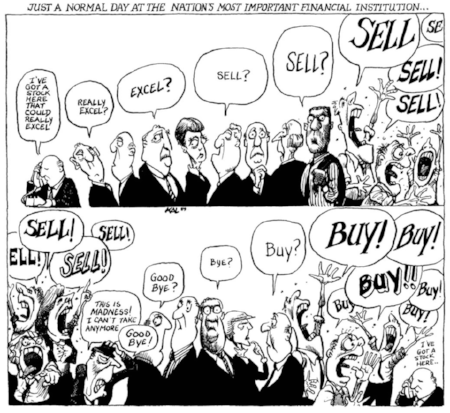
\includegraphics[width=.6\textwidth]{img/ch-investing/FOMOFUD.png}
    \caption{Fear, Uncertainty and Doubt (FUD) veranderd in Fear Of Missing Out (FOMO).}
    \label{fig:FOMOFUD}
    \end{figure}
    \medskip


%{Houd daarbij het volgende in gedachten: de prijs is wat je ervoor betaalt, en de waarde is wat je ervoor krijgt. Betaal een te hoge prijs en het mogelijke rendement wordt gedecimeerd. De waarde van bijvoorbeeld een aandeel is relatief ten opzichte van de inkomsten dat het zal genereren over de levensduur van het bedrijf. Deze waarde wordt vooral bepaald door alle toekomstige kasstromen te verdisconteren in een actuele waarde, de intrinsieke waarde. Wanneer je te hoog inkoopt (tegen een onhoudbaar prijsniveau) - zal het rendement dat ontstaat als activa terugvallen naar hun intrinsieke waarde in de loop der tijd eroderen. Koop daarom gulzig wanneer anderen bang zijn en wees voorzichtig wanneer anderen overenthousiast zijn. Zo maak je meer kans op winst. Met andere woorden: \say{buy high, sell low} \medskip }

\section{Macro trends}
Door meer kennis te vergaren word je minder snel be\"invloedt door emoties die op je af komen. Op de achtergrond spelen meer invloeden mee in de economie en maatschappij en we behandelen een aantal die van belang zijn wanneer je in markten begeeft.

    \begin{quotation}
      \textit{\say{History doesn't repeat itself, but it often rhymes}}
      \end{quotation}
   
\subsection{Economische cyclus}
De economische cyclus is de natuurlijke fluctuatie van de economie tussen perioden van expansie (groei) en krimp (recessie) \footnote{Investopedia; \href{https://www.investopedia.com/terms/e/economic-cycle.asp}{What is the Economic Cycle}}. Factoren zoals het bruto binnenlands product (BBP), de rentetarieven, het werkgelegenheidsniveau en de consumptieve bestedingen kunnen helpen om de huidige fase van de economische cyclus te bepalen. In tijden van expansie proberen investeerders bedrijven te kopen in technologie, kapitaalgoederen en primaire energiebronnen. In tijden van krimp proberen investeerders aandelen van ondergewaardeerde bedrijven, nutsbedrijven, financi\"ele instellingen en bedrijven in de gezondheidszorg te kopen.


       
\subsection{Bedrijfscyclus}
Bedrijfscyclussen vertegenwoordigen de stijging en daling van de productie van goederen en diensten in een economie. De conjunctuurcyclussen zijn de schommelingen in de economische activiteit binnen die economie, die zij gedurende vele jaren of decennia ondervindt. Deze schommelingen omvatten de productie van alle sectoren, met inbegrip van huishoudens, non-profitorganisaties (NGO's), overheden en andere bedrijfsoutput. Perioden van economische expansie en inkrimping kenmerken de conjunctuurcyclus. Tijdens een expansie beleeft de economie groei, terwijl een krimp (recessie) een periode van economische neergang of achteruitgang is. \Cref{fig:economiccycle1,fig:economiccycle2} de typische stadia van de bedrijfscyclus laten zien: expansie, piek, recessie of krimp, depressie, dieptepunt en herstel.
Sommige economen geloven dat de conjunctuurcyclus een natuurlijk onderdeel is van de economie. Anderen geloven dat centrale banken de cyclus indirect controleren en beïnvloeden door in te grijpen in het monetair beleid.



\begin{figure}
    \begin{minipage}{.5\textwidth}
        \centering
        \subcaption{cycle excluding growth trend}
        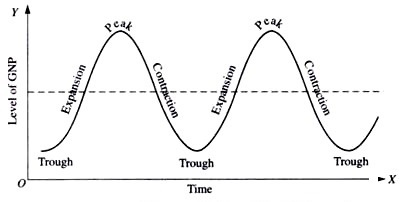
\includegraphics[width=\textwidth]{img/ch-investing/economic_cycle.jpg}
        \label{fig:economiccycle1}
    \end{minipage}
    \hfill
    \begin{minipage}{.5\textwidth}
        \centering
        \subcaption{cycle including growth trend}
        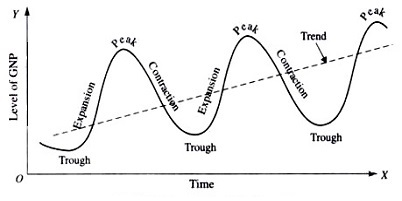
\includegraphics[width=\textwidth]{img/ch-investing/economic_cycletrend.jpg}
        \label{fig:economiccycle2}
    \end{minipage}  
    \label{fig:1-2}
  
    \caption{Cyclus met en zonder een algemene groei-trend}
    \source{Your Article Library; \href{http://www.yourarticlelibrary.com/macro-economics/theories-macro-economics/business-cycles-meaning-phases-features-and-theories-of-business-cycle/38063}{Knowledge Sharing Platform}.}
\end{figure}


\subsection{Kredietcyclus}
De kredietcyclus belichaamt de uitbreiding en inkrimping en vertegenwoordigt de toegang tot krediet in de loop van de tijd. Het beschrijft terugkerende fasen van gemakkelijk en moeilijk lenen en uitlenen binnen de economie. Sommige economen, waaronder Hyman Minsky en Steve Keen, beschouwen de kredietcyclus als het fundamentele proces dat de bedrijfs-cyclus aanstuurt. Een kredietcyclus beschrijft de fasen van toegang tot krediet voor kredietnemers. Krediet-cycli gaan eerst door periodes waarin de middelen relatief gemakkelijk te lenen zijn; lagere rentetarieven kenmerken deze periodes, dalende kredietbehoefte en een toename van de hoeveelheid beschikbaar krediet, wat een algemene uitbreiding van de economische activiteit stimuleert. Na deze periodes volgt een inkrimping van de beschikbaarheid van middelen. Tijdens de krimp van de kredietcyclus stijgen de rentetarieven en worden de regels voor kredietverlening strenger, wat betekent dat er minder krediet beschikbaar is voor zakelijke leningen, woningkredieten en andere leningen. De inkrimpingsperiode gaat door totdat de risico's voor de kredietverlenende instellingen zijn gereduceerd, op welk punt de cyclus afneemt en uiteindelijk opnieuw begint met hernieuwd krediet.

\section{Voorkom emotionele beslissingen}
Wat je ook wilt kopen, het zal er morgen nog steeds zijn, en misschien is het zelfs wel goedkoper. Wees dus te allen tijde bewust van het volgende en probeer bepaalde emoties niet te laten meespelen in al je keuzes:

\begin{enumerate}
    \item Als de markten zich bewegen, dan is dat ook het geval met het algemene marktsentiment. Mensen raken overenthousiast en zijn geneigd tot overdrijving. Herken de hype en leer winst te maken of riskeer alles te verliezen.
    \item Raak niet emotioneel gehecht aan je investering - je zult niet elke trade goed krijgen; neem het niet persoonlijk op. Streef altijd naar rationele keuzes, maar als je zich richt op de lange termijn, houd dan je beleggingskeuzes in lijn met je persoonlijke overtuigingen.
    \item Laat je niet scammen. Mensen kunnen hun redenen hebben om je in een bepaalde richting te sturen. Jouw niveau van due diligence is direct gerelateerd aan je vermogen om een potenti\"ele red flag te herkennen en te identificeren.
    \item Niet in paniek raken of toegeven aan een hype (FOMO - FUD). Denk rationeel na over je beslissingen, op basis van je analyse, die verder wordt onderbouwd door jouw eigen onderzoek.
\end{enumerate}

\begin{tipbox}{\textbf{Tip}}
 Probeer je emoties in bedwang te houden als je belangrijke beslissingen neemt. Blijf kritisch nadenken, stel een strategie op, en wees je bewust van de heersende markt-sentimenten en de marktpsychologie op dat moment.
\end{tipbox}